\documentclass[a4paper,12pt]{article}

% ----------------------------
% Pacchetti utili
% ----------------------------
\usepackage[utf8]{inputenc}
\usepackage[T1]{fontenc}
\usepackage[italian]{babel}
\usepackage{graphicx}
\usepackage{xcolor}
\usepackage{colortbl}
\usepackage{geometry}
\usepackage{setspace}
\usepackage{fancyhdr}
\usepackage{tikz}
\usepackage[colorlinks=true, linkcolor=blue, urlcolor=blue, citecolor=blue]{hyperref}
% ----------------------------
% Impostazioni pagina
% ----------------------------
\geometry{
    top=2cm,
    bottom=2cm,
    left=2cm,
    right=2cm
}

\setstretch{1.2}

% ----------------------------
% Dati personalizzabili
% ----------------------------
\newcommand{\Gruppo}{Atlas}
\newcommand{\Email}{\href{mailto:team9.atlas@gmail.com}{\textcolor{blue}{\underline{team9.atlas@gmail.com}}}}
\newcommand{\TitoloUno}{Dichiarazione degli impegni}
\newcommand{\DataModifica}{2025/10/29}
\newcommand{\LogoGruppo}{img/AtlasLogo.png} % Inserisci il file del logo

% --- Nuove variabili aggiunte ---
\newcommand{\VersioneDocumento}{v1.0} % <-- modifica qui la versione o ID
\newcommand{\Interno}{Interno} 

\pagestyle{fancy}
\fancyhf{}
\fancyhead[L]{\Gruppo}
\fancyhead[R]{Documento: \Interno \space - \space \DataModifica}
\fancyfoot[C]{\thepage}

% ----------------------------
% Inizio documento
% ----------------------------
\begin{document}

% ----------------------------
% Prima pagina
% ----------------------------
\begin{titlepage}
    \centering

    % Logo in alto
    \vspace*{0cm}
    \begin{tikzpicture}
        \clip (0,-0.1) circle (4.6cm); % raggio = metà della larghezza desiderata
        \node at (0,0) {\includegraphics[width=10cm]{\LogoGruppo}};
    \end{tikzpicture}\\[0.8cm]

    % Nome gruppo ed email sotto al logo
    {\LARGE \textbf{\Gruppo}}\\[0.1cm]
    {\large \Email}\\[1.2cm]

    % Sottotitolo del progetto
    {\Large \textit{Progetto di ingegneria del software A.A. 2025/2026}}\\[1.5cm]

    % Titolo principale
    {\Huge \textbf{\TitoloUno}}\\[.5cm]

    % Dati riunione
    \begin{tabular}{rl}
        \textbf{Data ultima modifica:} & \DataModifica \\
        \textbf{Versione:} & \VersioneDocumento \\
    \end{tabular}

\end{titlepage}


\section*{Tabella delle revisioni}
    \begin{center} 
        \begin{tabular}{|l|l|l|l|l|}
            \hline
            \textbf{Versione} & \textbf{Data} & \textbf{Autore} & \textbf{Verificatore} & \textbf{Descrizione} \\
            \hline
            v1.0 & 2025/10/29 & Riccardo Valerio & Andrea Difino & Correzione e modifica\\
            &&& Francesco Marcolongo & \\
            \hline 
            v0.2 & 2025/10/29 & Giacomo Giora & Francesco Marcolongo & Aggiunta contenuti \\
            \hline
            v0.1 & 2025/10/28 & Andrea Difino & & Prima Stesura \\
            \hline
        \end{tabular}
    \end{center}


\newpage

\tableofcontents

\newpage


\section{Introduzione}
Questo documento raccoglie la \textbf{dichiarazione degli impegni} del gruppo \textbf{Atlas}, che ha scelto di sviluppare il capitolato \textbf{C1 – Automated EN18031 Compliance Verification}, proposto da \textbf{Bluewind S.r.l.}.
Con questo documento intendiamo definire in modo chiaro la suddivisione delle ore di lavoro, i ruoli, i costi stimati e la pianificazione delle attività fino alla consegna del prodotto.

\section{Impegni orari e struttura dei costi}
Ogni componente del gruppo Atlas si impegna a contribuire con \textbf{91 ore produttive}, per un totale complessivo di \textbf{637 ore}.  
La suddivisione è stata pianificata per assicurare un equilibrio tra ruoli gestionali, analitici, progettuali e tecnici, mantenendo una proporzione coerente con le esigenze del progetto e con la sua complessità.

\begin{center}
\begin{tabular}{|l|c|c|c|c|c|}
    \hline
    \rowcolor{gray!20}
    \textbf{Ruolo} & \textbf{Costo/h}(\texteuro) & \textbf{Ore Totali} & \textbf{Ore/Membro} & \textbf{Costo}(\texteuro) & \textbf{\%} \\
    \hline
    Responsabile & 30 & 56 & 8  & 1680 & 8.8 \\
    \hline
    Amministratore & 20 & 70 & 10 & 1400 & 11.0 \\
    \hline
    Analista & 25 & 84 & 12 & 2100 & 13.2 \\
    \hline
    Progettista & 25 & 112 & 16 & 2800 & 17.5 \\
    \hline
    Programmatore & 15 & 168 & 24 & 2520 & 26.4 \\
    \hline
    Verificatore & 15 & 147 & 21 & 2205 & 23.1 \\
    \hline
    \rowcolor{gray!20}
    \multicolumn{2}{|c|}{\textbf{Totale}} & \textbf{637} & \textbf{91} & \textbf{12\,705} & \textbf{100} \\
    \hline
\end{tabular}
\end{center}

\begin{figure}[h]
    \centering
    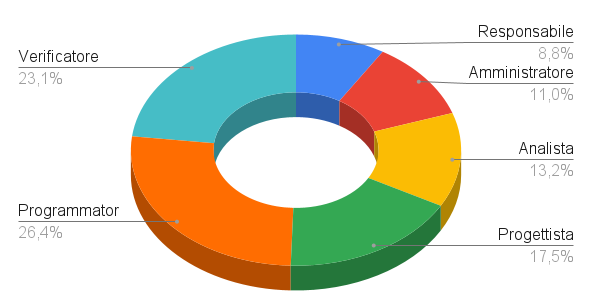
\includegraphics[width=14cm]{img/SuddivisioneRuoli.png}
    \caption{Ripartizione percentuale dei ruoli nel progetto}
\end{figure}

\newpage

\section{Descrizione dei ruoli}
La distribuzione dei ruoli nasce da una valutazione delle competenze presenti nel gruppo e dalle caratteristiche specifiche del progetto Bluewind, che richiede una forte attenzione alla qualità del codice, alla tracciabilità e alla verifica di conformità.

Il calcolo del monte ore per ruolo è avvenuto tenendo in considerazione le seguenti funzioni per i ruoli da ricoprire:
        
        \begin{itemize}
            \item \textbf{Responsabile}: Punto di riferimento per le comunicazioni con il committente. Deve riuscire ad anticipare l'evoluzione del progetto in modo da pianificare le attività, gestire il team e tenere sotto controllo i progressi. Ha responsabilità di scelta e approvazione, per cui è essenziale e partecipa per tutta la durata del progetto;
            \item \textbf{Amministratore}: Si occupa dell'efficienza e dell'operatività dell'ambiente di sviluppo, deve assicurarsi che in ogni istante le risorse siano presenti e operanti. Ha il compito di gestione del controllo della configurazione del prodotto, del versionamento e della documentazione di progetto e definisce procedure, strumenti e convenzioni;
            \item \textbf{Analista}: Si occupa di capire e formalizzare il problema in maniera chiara. Il suo lavoro ha grande impatto sulla riuscita del progetto, in quanto raccoglie i requisiti dal cliente, li analizza e li specifica in modo chiaro e verificabile;
            \item \textbf{Progettista}: Si occupa dello sviluppo della soluzione al problema presentato tramite le attività di progettazione. Traduce i requisiti in architettura e soluzioni tecniche, definisce la struttura del sistema e sceglie tecnologie, pattern, protocolli di comunicazione;
            \item \textbf{Programmatore}: Si occupa di implementare la soluzione trovata dal progettista in codice, realizzando concretamente il software, e di contribuire ai test unitari di ausilio alla verifica;
            \item \textbf{Verificatore}: Deve essere a conoscenza delle norme e deve avere capacità di giudizio e relazione con il codice sorgente in particolare e con il sistema in generale. Si occupa di attività di verifica e validazione, partecipando all'intero ciclo di vita e controllando che il prodotto rispetti i requisiti e sia di qualità attraverso i test.
        \end{itemize}

\section{Distribuzione delle ore}
La ripartizione delle ore è stata definita considerando le attività richieste dal capitolato \textbf{C1 – Automated EN18031 Compliance Verification}, proposto da \textbf{Bluewind S.r.l.}.  
Il progetto prevede la realizzazione di un sistema in grado di verificare automaticamente la conformità del software rispetto a specifiche norme di sicurezza e qualità. Questo tipo di progetto richiede particolare attenzione alla fase di progettazione, alla precisione dell’analisi iniziale e alla costante attività di verifica dei risultati.

\begin{itemize}
    \item \textbf{Responsabile – 56 ore:} le ore dedicate riflettono un impegno costante nel coordinare il gruppo, pianificare le attività e mantenere il contatto con il proponente. Il ruolo ha un peso moderato ma distribuito lungo l’intera durata del progetto, per garantire coerenza e continuità organizzativa.
    
    \item \textbf{Amministratore – 70 ore:} l’amministratore si occupa della gestione degli strumenti, del versionamento e dell’ambiente di lavoro condiviso. Il numero di ore previsto è proporzionato alla necessità di mantenere efficiente un’infrastruttura di sviluppo collaborativa e ben controllata.
    
    \item \textbf{Analista – 84 ore:} la fase di analisi è centrale, poiché il progetto richiede di comprendere e formalizzare requisiti tecnici e normativi. Le ore assegnate riflettono l’importanza di una definizione accurata dei requisiti funzionali e di vincolo, che guideranno le successive fasi di progettazione e sviluppo.
    
    \item \textbf{Progettista – 112 ore:} il ruolo del progettista assume particolare rilievo, in quanto è necessario definire un’architettura chiara, modulare e facilmente manutenibile. Le ore assegnate tengono conto della complessità strutturale del sistema e della necessità di tradurre i requisiti in soluzioni tecniche concrete.
    
    \item \textbf{Programmatore – 168 ore:} la parte di sviluppo costituisce la componente più corposa del progetto. Le ore sono state assegnate per coprire la realizzazione delle funzionalità principali, l’integrazione dei moduli e la scrittura del codice secondo gli standard di qualità richiesti.
    
    \item \textbf{Verificatore – 147 ore:} una quota significativa di ore è destinata alla verifica e validazione, attività fondamentali per un progetto che ruota attorno al concetto di conformità. Il verificatore dovrà controllare la correttezza dei prodotti sviluppati e assicurare che ogni fase rispetti i requisiti stabiliti. Il ruolo del verificatore ha un monte ore quasi pari a quello del programmatore in quanto il progetto C1 richiede la verifica di una grande quantità di decision tree.  
\end{itemize}

La distribuzione complessiva risponde quindi alle esigenze del capitolato, bilanciando le fasi di analisi, progettazione, sviluppo e verifica.  
In questo modo, ogni ruolo contribuisce in modo proporzionato al raggiungimento di un risultato finale affidabile, tracciabile e conforme agli obiettivi fissati.


\section{Rotazione dei ruoli}
    Le ore di lavoro verranno suddivise equamente tra i membri del gruppo, in modo da garantire che ciascuno possa ricoprire tutti i ruoli nel corso del progetto. È previsto un periodo di assegnazione del ruolo di due settimane, al termine del quale avverrà una rotazione e ciascun membro assumerà un ruolo diverso rispetto a quello svolto in precedenza, rispettando i vincoli di progetto. In questo modo, ogni membro del gruppo avrà l'opportunità di acquisire esperienza in ogni fase di ciclo di vita del software, migliorando le proprie competenze e contribuendo in modo più completo al successo del progetto, oltre che di valutarsi nello svolgimento dei vari ruoli.



\section{Preventivo e data di consegna}
Il gruppo \textbf{Atlas} prevede un impegno complessivo di \textbf{637 ore di lavoro}, corrispondenti a un costo totale stimato di \textbf{12\,705}\texteuro.  
La conclusione delle attività e la consegna del prodotto sono previste entro e non oltre il \textbf{20 marzo 2026}.
 

\end{document}
